%% LyX 2.2.2 created this file.  For more info, see http://www.lyx.org/.
%% Do not edit unless you really know what you are doing.
\RequirePackage{fix-cm}
\RequirePackage{fixltx2e}
\documentclass[english]{article}
\usepackage[T1]{fontenc}
\usepackage[latin9]{inputenc}
\usepackage{geometry}
\geometry{verbose,lmargin=2.5cm,rmargin=2.5cm}
\usepackage{babel}
\usepackage{array}
\usepackage{float}
\usepackage{textcomp}
\usepackage{pdfpages}
\usepackage{graphicx}
\usepackage{setspace}
\usepackage[unicode=true,pdfusetitle,
 bookmarks=true,bookmarksnumbered=false,bookmarksopen=false,
 breaklinks=false,pdfborder={0 0 1},backref=false,colorlinks=false]
 {hyperref}

\makeatletter

%%%%%%%%%%%%%%%%%%%%%%%%%%%%%% LyX specific LaTeX commands.
%% Because html converters don't know tabularnewline
\providecommand{\tabularnewline}{\\}
%% A simple dot to overcome graphicx limitations
\newcommand{\lyxdot}{.}


%%%%%%%%%%%%%%%%%%%%%%%%%%%%%% User specified LaTeX commands.
\usepackage{listings}
\usepackage{xcolor}
\usepackage{pdflscape}
\usepackage{courier}
%\usepackage{mathtools}
\usepackage{graphicx}
\usepackage{booktabs}
\usepackage[T1]{fontenc}
\usepackage{lmodern}

\usepackage{listings}
\lstset{columns=fullflexible}

\usepackage{charter}

\usepackage{xspace}



% Definizione intestazioni e pie' di pagina
\usepackage{fancyhdr}

\makeatother

\begin{document}
\begin{titlepage}


\newcommand{\HRule}{\rule{\linewidth}{0.5mm}}
\center
\textsc{\LARGE Politecnico di Milano}\\[1.5cm] \textsc{\Large PowerEnjoy}\\[0.5cm]
\textsc{\Large Software Engineering 2}\\[0.5cm]

\HRule \\[0.4cm] { \huge \bfseries Requirements Analysis and \\ Specification Document}\\[0.4cm] \HRule \\[1.5cm]
\begin{minipage}{0.4\textwidth} \begin{flushleft} \large \emph{Authors:}\\ Giancarlo \textsc{Colaci} \newline Giulio \textsc{De Pasquale} \newline Francesco \textsc{Rinaldi} \end{flushleft} \end{minipage} ~ \begin{minipage}{0.4\textwidth} \begin{flushright} \large \emph{Supervisor:} \\ Elisabetta \textsc{De Nitto} \end{flushright} \end{minipage}\\[3cm]

\includegraphics[width=0.3\textwidth]{res/img/logopm}

\vfill
{\large \today}\\[3cm]

\end{titlepage}\newpage{}

\mbox{} \thispagestyle{empty} \newpage

\newpage{}

\tableofcontents{}\thispagestyle{empty}\newpage{}

\mbox{} \thispagestyle{empty} \newpage

\newpage{}

\setcounter{page}{1}

\section{Introduction}

\subsection{Description of the given problem }

We will project and implement PowerEnjoy, which is a new car-sharing
service that exclusively employs electric cars. The system that will
be developed has to allow the registration of a new user with all
his personal information (like name, age, driving license and credit
card information), log in credentials and the possibility to find
the locations of available cars within a certain distance from his
current location or from a specified address. Moreover, according
to some policies (specified later) the user can obtain exclusive discounts
and offers.

\subsection{Purpose}

The principal purpose of this document, the Requirement Analysis and
Specification Document, is to show the functional and non-functional
requirements of the system-to-be. They will be based on different
aspects: the needs expressed by the stakeholders, the constraints
which it is subject to, the typical scenarios that will happen after
its deployment. The targeted audience in this case will be mainly
made of software engineers and developers who have to actually develop
the service here described.

\subsection{Scope}

The system will be an optimization of a pre-existing system for renting
electric cars already in use in some cities. The new system will let
users to check reservability and status of available cars, rent or
reserve them through a mobile or a web application in a more simple
and effective way. In addition to a better user interface, the new
system will guarantee a smarter uniform distribution of cars in the
city, in order to offer a better service for the citizens, and will
also offer some special discount, in order to incentivize the virtuous
behaviors of the users.

\subsection{Goals }

PowerEnJoy's users will be able to:
\begin{itemize}
\item register themselves to the system;
\item log into the system;
\item find the location of available cars in a specified area;
\item book a car with the possibility to cancel the reservation;
\item open his / her reserved car;
\item be notified of active reservation status;
\item end the rental;
\item know the total cost at the end of the lease;
\end{itemize}

\subsection{Stakeholders}

Our primary stakeholder is the professor who gave us this didactical
project. Our stakeholder's main need is to review the complete project
at the end of the semester. Our objective is to show him/her we have
followed the development process in all its parts and that we are
able to carry out a challenging task from the beginning to the end
fully comprehending all its internal phases. We want to show that
we can identify key requirements and specifications, design and test
our web/mobile application while providing all documentation backing
up the source code. Finally, our typical users will be people that
don\textquoteright t have a car or that prefer to rent a car instead
of a public service transportation to go around the city.

\subsection{Glossary}

Below there are definitions of some terms that will be used in the
document, in order to avoid any ambiguity in their use and their understanding.
\begin{description}
\item [{Guest:}] a person that has never signed up to the system. He can
only sign up and view available cars
\item [{User:}] a person already registered in the system who can log in
and has a personal profile and can use all the functionalities described.
Unless specified, each user is active: therefore can use the service
with no restrictions
\item [{Deactivated~user:}] a user with revoked privileges. He/she cannot
use the service until the issues with his/her account are solved (e.g.,
expired license)
\item [{Login:}] the action of accessing the system via a username and
related password
\item [{Notification:}] a real-time alert that warns a user when there
are updates about what he is dealing with
\item [{Reservation:}] the action performed by the registered user when
he chooses to drive an available car. It expires as soon as one of
these conditions is met: one hour is elapsed from the user's reservation
request or the car is unlocked
\item [{Rent:}] the temporary possession and use of one of the PowerEnjoy's
cars in return for payment by a user. It starts once a minute is elapsed
from the car doors unlock or the engine is ignited and lasts until
the doors are re-locked by the system
\item [{Available:}] a fully functional car ready to be used by a registered
user
\item [{Unavailable:}] a car which is currently reserved or used by a registered
user or is not entirely working (e.g. exhausted battery, mechanical
damage)
\item [{Reservable:}] an available car located in a geographical region
where a registered user is enabled to reserve it
\item [{Parking~area:}] circumscribed public area where cars can be parked
(e.g. no parking lots). The set of safe areas for parking cars is
pre-defined by the management system.
\item [{Recharging~area:}] it is included in the parking area; cars parked
here can also be recharged thanks to several charging stations
\item [{Special~area:}] specific recharging areas decided by the system
to ensure a uniform distribution of cars in the city
\item [{RMSS:}] Request Management Sub-System, it is an already developed
part of our system which stores and manages all the information about
the PowerEnjoy's cars, users and about their request (reservation
or rent).
\item [{MES:}] Maintenance External Service, it is an external service
that takes care of ordinary or extraordinary car maintenance.
\item [{ADS:}] Auto Diagnosis System, an always on embedded peripheral
which continuously monitors the status of the car (e.g. battery charge,
tires pressure, impact detection)
\item [{ECS:}] Emergency Call System, an always on embedded peripheral
which can be used to call the consumer service or an emergency number
quickly
\item [{Verification~code:}] it is a four digits code chosen by the user
during the registration procedure that adds another level of security
to our service; the user will need it to unlock the car
\item [{Countdown:}] it is the time given to the user to pick-up the reserved
car before the reservation expires (during this period the reservation
is active)
\item [{EULA:}] End User License Agreement
\end{description}
\newpage{}

\section{Overall Description}

\subsection{Proposed System}

The server-side implementation will be structured through a net of
micro-services mainly written in Python and managed through Docker.
The server will run the business logic, host PowerEnjoy's website,
and users' data. Besides, we propose a web/mobile application which
allows to registered users to use PowerEnjoy's services. The web client
will use Python/Javascript and HTML5/CSS for web pages generation
and formatting respectively. We will also use open-source libraries
such as Flask to speed up the development. The mobile applications
will be deployed on the main platforms currently available (iOS, Android,
Windows Phone) and will be written accordingly to each devices' programming
language. Client-server communication will be platform agnostic since
it will happen through an encrypted RESTful API which returns its
data through JSON.

\subsection{Domain Properties}

We suppose these conditions will be respected at any given time:
\begin{itemize}
\item the user will request help only if he/she needs it;
\item the user will never try to exploit the system's features (e.g. sleep
in the car);
\item the user will never fake his/her position to cause a denial of service; 
\item the user will only provide correct and authentic information while
signing up
\item a booked car will always be driven by the user who reserved it;
\item the user will never be robbed of the access credentials and the verification
code;
\item the user agrees to be geolocalized;
\item each available car is fully functional;
\item each car has an embedded key to turn on the engine;
\item each car is equipped with a properly working ADS and an ECS;
\item each car is fitted with a properly working notification touchscreen
display;
\item an available car will always be found in the supposed position;
\end{itemize}
\pagebreak{}

\subsection{Assumptions}

This section explores some of the vague concepts or loosely explained
ones: further hypotheses have been added to expand the description
of the requirements and to account better for the interaction between
the external environment and the developed application.

Due to some unclear points in the specification we made some assumptions,
which are: 
\begin{itemize}
\item the system allows users to locate any car in PowerEnjoy's area of
operation;
\item the system's money saving option has to be enabled or disabled in
the user profile;
\item the system permits users to reserve an available car only in his/her
city;
\begin{itemize}
\item with \textquotedbl{}a certain geographical region\textquotedbl{} we
mean that the user can reach the vehicle in a reasonable amount of
time;
\end{itemize}
\item the system can locate its users through Cellular Data or GPS; 
\item the system's proximity check is done through one of these: numerical
code on each cars' windshield or GPS data from user's phone;
\item the fees are applied as soon as one of these conditions is met: one
minute is elapsed from the car's doors opening, or the engine is revved;
\item each seat is equipped with a sensor which is used to detect the number
of passengers into each car;
\item each user can't reserve more than one car at the same time;
\item to be eligible for the 10\% discount, almost two passengers have to
remain seated at the same time for at least one minute;
\item if a car is parked in a special area, the discount equals to 40\%;
\end{itemize}

\subsection{Actors Identifying}

The system provides the interaction of two different types of actors
who can use different functionalities of the application system. The
types are set out below along with a brief description of their privileges.

\subsubsection{Guest}

A person that is not registered (yet!) so can check for cars' position,
register or ask for help/advice.

\paragraph{Privileges:}
\begin{itemize}
\item Register to the system by creating a new account;
\item Check available cars' position and status;
\item Contact the customer service;
\end{itemize}

\subsubsection{User}

A person that is already registered to the system with his personal
information; a guest can become a user after the authentication to
the system using the login form.

\paragraph{Privileges:}
\begin{itemize}
\item Log into the system;
\item Consult reservations' history;
\item Edit account information:
\begin{itemize}
\item personal and billing data;
\item enable/disable money saving option; 
\end{itemize}
\item Check available cars' position and status;
\item Reserve a reservable car;
\item Rent the reserved car;
\item Check active reservation status:
\begin{itemize}
\item Remaining time until the reservation expires;
\item Reserved car's position and status;
\item Elapsed rental time;
\end{itemize}
\item Request help through the ECS;
\item Terminate the rent;
\item Contact the customer service;
\end{itemize}

\subsubsection{Deactivated User}

A user with revoked privileges. He/she cannot use the service until
the issues with his/her account are solved (e.g expired license).

\paragraph{Privileges:}
\begin{itemize}
\item Log into the system;
\item Consult reservations' history;
\item Edit account information:
\begin{itemize}
\item personal and billing data;
\item enable/disable money saving option; 
\end{itemize}
\item Check available cars' position and status;
\item Contact the customer service;
\end{itemize}
\newpage{}

\section{Specific Requirements}

In this section will be analyzed in detail functional and non-functional
requirements that the system developed has to satisfy, when the domain
properties previously denoted hold and referring to the declared goals.

\subsection{Functional requirements}

The functional requirements include the functionalities that the system
must necessarily have and describe the interactions between the system
developed and the external environment independently from the implementation.
\begin{enumerate}
\item Registration of a guest to the system:
\begin{enumerate}
\item The system has to guarantee the registration to a new user by creating
a new account.
\end{enumerate}
\item Login of a user into the system:
\begin{enumerate}
\item The system has to allow the login to an already registered user when
he types the correct username and the password in the login form.
\end{enumerate}
\item Find the location of available cars in a specified area:
\begin{enumerate}
\item The system has to allow both guests and users to specify the address
where they want to locate an available car or to use their position;
\item The system has to guarantee that a car is showed on the map if and
only if it is available (that means that every available car is showed
and that every showed car is available);
\item The system has to guarantee that the car's position is regularly showed
up to date.
\end{enumerate}
\item Book a car with the possibility to cancel the reservation:
\begin{enumerate}
\item The system has to guarantee that only a user (i.e. not a guest) can
reserve a car;
\item The system must be able to check the position of the user;
\item The system has to guarantee that any user can reserve only one car
at a time;
\item The system has to ensure that the same car cannot be reserved at the
same time by different users;
\item The system has to guarantee that any user can have at most an active
reservation;
\item The system has to guarantee that every reservable car is available;
\item The system has to ensure that only a reservable car can be reserved;
\item The system has to guarantee that when a user reserves a car, the latter
is no more available;
\item The system has to ensure that only an active reservation can expire
or be canceled;
\item The system has to make sure that when a reservation expires or is
revoked, the car becomes available again;
\item When a reservation is activated, the system starts a countdown at
the end of which the reservation expires if the user did not pick-up
the reserved car;\pagebreak{}
\end{enumerate}
\item Open his/her reserved car;
\begin{enumerate}
\item The system must be able to check the proximity of the user to the
reserved car;
\item The system must be able to check if the money saving option is enabled
for the current reservation;
\item The system has to allow the user to insert the verification code;
\item The system has to unlock the reserved car only if the entered verification
code is correct;
\end{enumerate}
\item Be notified of active reservation status:
\begin{enumerate}
\item The system must be able to retrieve the starting time of the rental;
\item The system must be able to calculate and notify the elapsed time of
the rental periodically;
\item The system must be able to communicate with every grid power station
to check their power plugs' availability;
\item The system, to ensure a uniform distribution of parked cars, must
be able to notify the user the nearest selected station where to leave
the car to get a discount only if he/she inputs a destination and
the money saving option is active; 
\end{enumerate}
\item End the rental:
\begin{enumerate}
\item The system has to allow the user to communicate that he/she wants
to terminate the rental using the car's display;
\item The system has to allow the user to end the rental only if he is in
a safe parking area;
\item The system has to guarantee that when a reservation is ended, the
car becomes available again;
\end{enumerate}
\item Know the total cost at the end of the rental:
\begin{enumerate}
\item The system has to communicate with the ADS to retrieve the car status
and rental information;
\item The system must be able to apply the discounts, if any, handling the
previously retrieved information;
\item The system must communicate to the user the final cost of the rental;
\end{enumerate}
\end{enumerate}

\subsection{Non-functional requirements }

The non-functional requirements are those not related to the functionality,
but rather consider the quality of the system to be implemented (Quality
of Service, QoS), regardless of the application domain. 

Security:
\begin{itemize}
\item Each user will only be able to access functionality that competes
to his category, and it is, therefore, necessary to provide an authentication
method: it will be used the symmetric username/password one. Furthermore,
each credential will not be stored in cleartext, and client/server
communications will be protected by asymmetric encryption. 
\end{itemize}
Portability: 
\begin{itemize}
\item The client must be compatible with all hardware and software platforms
to reach as many users as possible. This requirement is satisfied
by realizing the client as a web application, in this way the only
assumptions that must be met by users are the availability of a web
browser and a connection to the Internet. 
\end{itemize}
Stability and reliability: 
\begin{itemize}
\item The system must notify the user the result of each his/her transaction
request while maintaining an optimal level of reliability. Therefore
it will be able to face with the possible loss of connection between
clients and the central server by ensuring atomicity of all operations.
\end{itemize}
Performance: 
\begin{itemize}
\item As for performance, the timing of getting and insertion the information
in the database must be acceptable to do not block the whole system. 
\end{itemize}
Concurrency management: 
\begin{itemize}
\item The system must ensure data consistency while dealing with multiple
concurrent accesses to the same resource in the database by multiple
users authenticated to the system. 
\end{itemize}
Graphical User Interfaces (GUIs): 
\begin{itemize}
\item The system has to include several graphical user interfaces: intuitive,
complete and exceptionally easy to use. An interface to contain areas
of input, dialog boxes, buttons, links and drop-down menus will be
developed. The interfaces will interact with business logic and then
be differentiated according to user roles in the system: each interface
will provide access to features that compete for the particular user
who is logged in.
\end{itemize}
\newpage{}

\section{Scenarios}

This section will present some possible situations that may occur
from the interaction between a user and the system developed.

\quad{}

\subsection{Alice is curious about PowerEnjoy}

Lily tells Alice about a new service called PowerEnjoy: Alice, now
curious, tries to register to PowerEnjoy. She visits the homepage,
browses the site a little and then proceeds to the registration page.
Alice then enters all the data needed by the system to complete the
process: name and surname, username, email address, password, ID card
number and license number. To complete the sign-up she finally enters
the billing information. Once everything is done, the system sends
her a confirmation mail with a link used to activate her new account.
She has now completed the registration, and she can log into the system
and power enjoy the service.

\quad{}

\subsection{Grandpa Peter and his expired license}

Grandpa Peter has been registered to PowerEnjoy for a quite long time.
He loves the car sharing model, now more than ever since his old Panda
broke a long time ago and he could not pick up his nephews, David
and Goliath, from the pool. There is a problem, though: Peter is getting
old, and his license has to be renewed to drive again. After a long
day at the Driver and Vehicle Licensing Agency, Grandpa Peter successfully
got his shiny license back! To reactivate his PowerEnjoy account,
Peter has to edit his account data and insert the new license card
number: after having logged in, he proceeds to his personal area by
clicking \textquotedblleft Edit Personal Data\textquotedbl{}, he puts
the new data in the system, and finally he saves the changes. Grandpa
Peter is on the road, again!

\quad{}

\subsection{Grandpa Peter and his nephews}

It's rainy outside, so Grandpa Peter has to pick up his two nephews
from the pool: he picks up his smartphone and checks if there are
any available cars near him. He is getting old so he cannot walk for
a long time, so he reserves the nearest car which, unfortunately,
has less than 50\% battery charge remaining. Once in the car's reach,
Peter taps on \textquotedblleft Open Vehicle\textquotedblright{} and
inputs his verification code. His memory is aging just like him so
the usual \textquotedblleft 1969\textquotedblright{} code, which corresponds
to the year he married his beloved Franca, turned into \textquotedblleft 1967\textquotedblright{}
which is not accepted by the system. The system prompts him again,
and this time Peter does not fail: the doors unlock, and Grandpa is
on the road once more! Peter's driving skills are still amazing: he
picks up the kids and gets home in no time, so he ends the rent. Unfortunately,
he is not able to use the 20\% discount due to the battery charge
left, but he will be cut 10\% since he took at least two other people
in the car.

\pagebreak{}

\subsection{Pablo and Tata go to the cinema}

Tata and Pablo make a great couple. It's Friday night, and the theaters
are flooded by the latest sci-fi movie everyone love. Pablo loves
all those lightsabers and starships while Tata just can't get the
point out of them. The film will start in more than one hour: Pablo
is ready for the night out, Tata has to fix her makeup. \textquotedblleft Five
minutes and I am ready!\textquotedbl{} - she said. Unfortunately,
Pablo forgot to charge his phone so he can't use his phone's GPS to
save precious battery juice and reserves his PowerEnjoy car by entering
his address into the app. Time goes by; one hour has passed, and Pablo
is still waiting for Tata who seems to have no intentions leaving
the bathroom. The film has just begun, the reservation expired, the
car is available to be reserved again, and Pablo has to pay 1� fee:
\textquotedblleft One minute and we are rolling!\textquotedblright{}
- she said. Pablo, may the force be with you! 

\quad{}

\subsection{Gustavo, the discount hunter}

Gustavo is a saver, methodic and old-fashioned man, and he built an
economic empire from scratch. He owns a vintage 1968 Ford Torino which
is only used on Saturday afternoons with his closest friend to honor
the times long gone: on the other days, he mainly uses PowerEnjoy.
Gustavo has turned on the money saving option while signing up, and
he loves it. Once in the car, he logs in and proceed to set up his
seat and insert his destination: the system now calculates the overall
cars distribution in the city, verifies the availability of power
plugs in the nearest power grid stations to the arrival and suggests
to park in a special area just 300 meters away from his destination.
Once there, Gustavo, just before ending the rental, takes care of
plugging the car into the power grid: now, the smartphone application
shows him the total cost which includes the 40\% discount.

\newpage{}

\section{Models }

In this section we are going to abstract from the previously seen
scenarios in order to have a more high-level description. For this
purpose we will use UML (Unified Modeling Language) diagrams. 

\subsection{Use cases model }

From previously denoted scenarios and from the whole analysis we did
in this document, we individuated the use cases of the system to be
developed. In these pictures there are some use Cases diagram which
represent actors, their use cases and their interactions. Then some
of them are better explained using a less formal and more narrative
way.

\begin{figure}[H]
\begin{centering}
\includegraphics[width=0.6\textwidth]{res/img/Usecase_guest}
\par\end{centering}
\caption{Guest Use Case}
\end{figure}

\begin{figure}[H]
\begin{centering}
\includegraphics[width=1\textwidth]{res/img/usecase_user}
\par\end{centering}
\caption{User Use Case}
\end{figure}

\begin{figure}[H]
\begin{centering}
\includegraphics[width=1\textwidth]{res/img/Usecase_disuser}
\par\end{centering}
\caption{Deactivated User Use Case}
\end{figure}

\newpage{}

\subsubsection{Registration}

\begin{tabular}{>{\centering}p{0.2\textwidth}m{0.75\textwidth}}
\hline 
Actors & \vspace{0.15cm}Guest\vspace{0.15cm}\tabularnewline
\hline 
Preconditions & \vspace{0.15cm}The guest has a working Internet connection and he
has not registered an account yet.\vspace{0.15cm}\tabularnewline
\hline 
Events & \begin{enumerate}
\item The guest reaches the registration page 
\item The system requires the guest to enter all his/her personal information,
driving license data and login credentials along with the verification
code
\item The guest types the requested information and presses the \textquoteright Next\textquoteright{}
button
\item The system verifies the uniqueness of the email, the equality of the
twice typed passwords and that the driving license is not expired
yet
\item The system notifies the guest that he is going to be redirected to
an external service web page where he will be required to enter his
billing information
\item The system receives a confirmation from the external payment service
about the correctness of the billing information
\item The system shows to the guest a recap of the information already provided
and requires him to confirm them, to read and accept the EULA and
complete the registration
\item The guest ticks the \textquotedblleft I read carefully, and I accept
the contract\textquotedblright{} box and presses the \textquotedblleft Confirm
and Complete Registration\textquotedblright{} button
\item The system sends an email to notify the correct registration to the
guest
\item The system reports the registration and redirects the user to the
login page
\end{enumerate}
\tabularnewline
\hline 
Postconditions & \vspace{0.15cm}The user has signed up.\vspace{0.15cm}\tabularnewline
\hline 
Exceptions & \vspace{0.15cm}The email the guest typed has been already used. The
second password does not match with the first one. One of the fields
is empty. The SSN is not in compliance with the other guest's personal
information. The driving license is already expired. The external
payment service didn't confirm the billing information. The guest
did not accept the EULA. In these cases the system notifies the error
and cannot complete the registration.\vspace{0.15cm}\tabularnewline
\hline 
\end{tabular}

\subsubsection{Log in}

\begin{onehalfspace}
\begin{tabular}{>{\centering}p{0.2\textwidth}m{0.75\textwidth}}
\hline 
Actors & \vspace{0.15cm}User or Deactivated User\vspace{0.15cm}\tabularnewline
\hline 
Preconditions & \vspace{0.15cm}The actor has a working Internet connection and he
has already registered his account.\vspace{0.15cm}\tabularnewline
\hline 
Events & \begin{enumerate}
\item The actor reaches the log in page 
\item The system requires the actor to enter his email and password 
\item The actor types the requested information and press the \textquoteright Log
in\textquoteright{} button
\item The system verifies the correctness of the email and password
\item The system redirects the actor to his personal page
\end{enumerate}
\tabularnewline
\hline 
Postconditions & \vspace{0.15cm}The actor is logged in.\vspace{0.15cm}\tabularnewline
\hline 
Exceptions & \vspace{0.15cm}The email or the password the actor typed are not
correct. One of the fields is empty. In these cases the actor can\textquoteright t
complete the log in. The system notifies the error and cannot complete
the login.\vspace{0.15cm}\tabularnewline
\hline 
\end{tabular}
\end{onehalfspace}

\subsubsection{Edit personal information}

\begin{onehalfspace}
\begin{tabular}{>{\centering}p{0.2\textwidth}m{0.75\textwidth}}
\hline 
Actors & \vspace{0.15cm}User or Deactivated User\vspace{0.15cm}\tabularnewline
\hline 
Preconditions & \vspace{0.15cm}The actor has a working Internet connection and he
is already logged into the system.\vspace{0.15cm}\tabularnewline
\hline 
Events & \begin{enumerate}
\item The actor reaches his personal area
\item The actor clicks the ``Edit personal information'' button
\item The system allows the actor to change his address, mobile phone number,
password (and to confirm it), driving license number, the expiration
date and the authority who released it
\item The user enters the new information and presses \textquoteright Save\textquoteright{}
\item The system verifies the correctness and the completeness of the information
\item The system shows the actor his updated information
\end{enumerate}
\tabularnewline
\hline 
Postconditions & \vspace{0.15cm}The user has modified his personal information.\vspace{0.15cm}\tabularnewline
\hline 
Exceptions & \vspace{0.15cm}One of the fields is empty. The second password does
not match with the first one. The driving license is already expired.
In these cases the system notifies the error and cannot complete the
request.\vspace{0.15cm}\tabularnewline
\hline 
\end{tabular}
\end{onehalfspace}

\subsubsection{Edit billing information}

\begin{onehalfspace}
\begin{tabular}{>{\centering}p{0.2\textwidth}m{0.75\textwidth}}
\hline 
Actors & \vspace{0.15cm}User or Deactivated User\vspace{0.15cm}\tabularnewline
\hline 
Preconditions & \vspace{0.15cm}The actor has a working Internet connection and he
is already logged into the system.\vspace{0.15cm} \tabularnewline
\hline 
Events & \begin{enumerate}
\item The actor reaches his personal area
\item The actor clicks the ``Edit billing information'' button
\item The system notifies the actor that he is going to be redirect to an
external service web page where he will be required to enter his new
billing information
\item The system receives a confirmation from the external payment service
about the correctness of the new billing information
\item The system shows the actor his updated information
\end{enumerate}
\tabularnewline
\hline 
Postconditions & \vspace{0.15cm}The user has modified his billing information.\vspace{0.15cm}\tabularnewline
\hline 
Exceptions & \vspace{0.15cm}The external payment service did not confirm the billing
information. In this case the system notifies the error and cannot
complete the request.\vspace{0.15cm}\tabularnewline
\hline 
\end{tabular}
\end{onehalfspace}

\subsubsection{Check available cars' position and status}

\begin{onehalfspace}
\begin{tabular}{>{\centering}p{0.2\textwidth}m{0.75\textwidth}}
\hline 
Actors & \vspace{0.15cm}Guest, User or Deactivated User\vspace{0.15cm}\tabularnewline
\hline 
Preconditions & \vspace{0.15cm}The actor has a working Internet connection.\vspace{0.15cm}\tabularnewline
\hline 
Events & \begin{enumerate}
\item The actor opens the map
\item The system requires the actor to enter an address or to use his position
to localize cars 
\item The actor types the address where he wants to find an available car
or clicks ``Use my position'' button
\item The system verifies the correctness of the information and send a
request to the RMSS 
\item The system receives an answer from the RMSS with the available cars
and shows them to the actor on the map
\item The actor taps the icon that stands for the available car he chooses 
\item The system shows to the actor the status of the selected available
car
\end{enumerate}
\tabularnewline
\hline 
Postconditions & \vspace{0.15cm}The actor obtains all the information about the position
and the status of any available car in a certain area.\vspace{0.15cm}\tabularnewline
\hline 
Exceptions & \vspace{0.15cm}The address field is empty. The inserted address is
not found or the location service does not work. There is no available
cars in the selected area. In these cases the system notifies the
error and cannot complete the request.\vspace{0.15cm}\tabularnewline
\hline 
\end{tabular}
\end{onehalfspace}

\subsubsection{Reserve a car}

\begin{onehalfspace}
\begin{tabular}{>{\centering}p{0.2\textwidth}m{0.75\textwidth}}
\hline 
Actors & User\tabularnewline
\hline 
Preconditions & \vspace{0.15cm}The user has a working Internet connection, he has
already checked the position and the status of an available car and
he is logged into the system for the whole reservation.\vspace{0.15cm}\tabularnewline
\hline 
Events & \begin{enumerate}
\item The user clicks on \textquotedblleft Reserve car\textquotedblright{}
button
\item The system send to the RMSS the user position and his reservation
request 
\item The system receives an affirmative answer from the RMSS 
\item The system creates a new instance of the reservation 
\item The system notifies the user the success of the reservation
\end{enumerate}
\tabularnewline
\hline 
Postconditions & \vspace{0.15cm}The user reserved successfully a car.\vspace{0.15cm}\tabularnewline
\hline 
Exceptions & \vspace{0.15cm}The communication with the RMSS failed. The system
says to the user that the service is temporarily not available. The
localization service does not work. The system receives a negative
answer from the RMSS. In these cases the system notifies the error
to the user and he cannot complete the reservation.\vspace{0.15cm}\tabularnewline
\hline 
\end{tabular}
\end{onehalfspace}

\subsubsection{Open the reserved car}

\begin{onehalfspace}
\begin{tabular}{>{\centering}p{0.2\textwidth}m{0.75\textwidth}}
\hline 
Actors & User\tabularnewline
\hline 
Preconditions & \vspace{0.15cm}The user has a working Internet connection, has already
reserved a car and he is logged into the system.\vspace{0.15cm}\tabularnewline
\hline 
Events & \begin{enumerate}
\item The user reaches the car he reserved. 
\item The system checks user position or requires him to enter the code
on the windshield 
\item If necessary, the user enters the code he can read on the windshield
\item The system requires the user enter his verification code 
\item The user types his verification code 
\item The system verifies the correctness of the verification code and the
status of the reservation
\item The system unlocks the car doors, terminates the reservation and creates
a rent instance on the RMSS
\item The user opens the car doors 
\end{enumerate}
\tabularnewline
\hline 
Postconditions & \vspace{0.15cm}The user can get in the car.\vspace{0.15cm}\tabularnewline
\hline 
Exceptions & \vspace{0.15cm}The user failed to unlock the car in less than one
hour: the system notifies the end of the reservation to the user,
declares the reserved car as available again and applies 1� of fee
to the user. | The system is not able to check the user position.
The user fails to enter the windshield code. The verification code
is not correct. In these cases the system doesn\textquoteright t unlock
the doors.\vspace{0.15cm}\tabularnewline
\hline 
\end{tabular}
\end{onehalfspace}

\subsubsection{Use the reserved car and terminate the rent}

\begin{onehalfspace}
\begin{tabular}{>{\centering}p{0.2\textwidth}m{0.75\textwidth}}
\hline 
Actors & User\tabularnewline
\hline 
Preconditions & \vspace{0.15cm}The user has a working Internet connection, has already
opened his reserved car and he is logged into the system.\vspace{0.15cm}\tabularnewline
\hline 
Events & \begin{enumerate}
\item If the money saving option is actived, the user can enter his final
address on the touchscreen display in the car
\item If the user did it, the system shows a special parking area near his
destination
\item The user starts the engine and uses the car 
\item As a matter of choice, the user takes care of plugging the car into
the power grid
\item The user clicks ``Terminate rent''
\item The system verifies nobody is in the car and that it is in a safe
parking area
\item The system locks the car doors again, verifies the car's status and
updates the rent instance
\item If necessary, the system contacts the MES for an ordinary (or extraordinary)
car maintenance.
\item The system calculates the total cost and notifies the end of the rental
to the user along with the total cost
\end{enumerate}
\tabularnewline
\hline 
Postconditions & \vspace{0.15cm}The user successfully rented a car.\vspace{0.15cm}\tabularnewline
\hline 
Exceptions & \vspace{0.15cm}The address is not correct or it is not found. The
system notifies the error to the user and requires him to insert it
again. | The car is not in a safe parking area. The car is not empty.
In these cases the system doesn\textquoteright t allow to terminate
the rent. | The user can't pay the total cost: the system deactivate
the user.\vspace{0.15cm}\tabularnewline
\hline 
\end{tabular}
\end{onehalfspace}

\subsubsection{Contact customer service}

\begin{onehalfspace}
\begin{tabular}{>{\centering}m{0.2\textwidth}m{0.75\textwidth}}
\hline 
Actors & Guest, User or Deactivated User\tabularnewline
\hline 
Preconditions & \vspace{0.15cm}The actor has a working Internet connection.\vspace{0.15cm}\tabularnewline
\hline 
Events & \begin{enumerate}
\item The actor reaches the \textquotedblleft Contact the Customer Service\textquotedblright{}
page 
\item The system requires the actor to enter his own name, surname, mobile
phone number, email address and to explain his problem in less than
1000 words
\item The user types the requested information and press the \textquoteleft Contact
the Customer Service\textquotedblright{} button 
\item The system redirects the request of the user to the customer service.
\end{enumerate}
\tabularnewline
\hline 
Postconditions & \vspace{0.15cm}The actor successfully contacted the customer service.\vspace{0.15cm}\tabularnewline
\hline 
Exceptions & \vspace{0.15cm}The actor uses more than 1000 words to explain his
request. There is at least one empty field. In these cases the system
notifies the error and cannot complete the request.\vspace{0.15cm}\tabularnewline
\hline 
\end{tabular}
\end{onehalfspace}

\newpage{}

\subsection{Sequence Diagram}

This section presents the sequence diagram of the most important interaction,
in order to have a dynamic sight of the main entities too.

\begin{figure}[H]
\begin{centering}
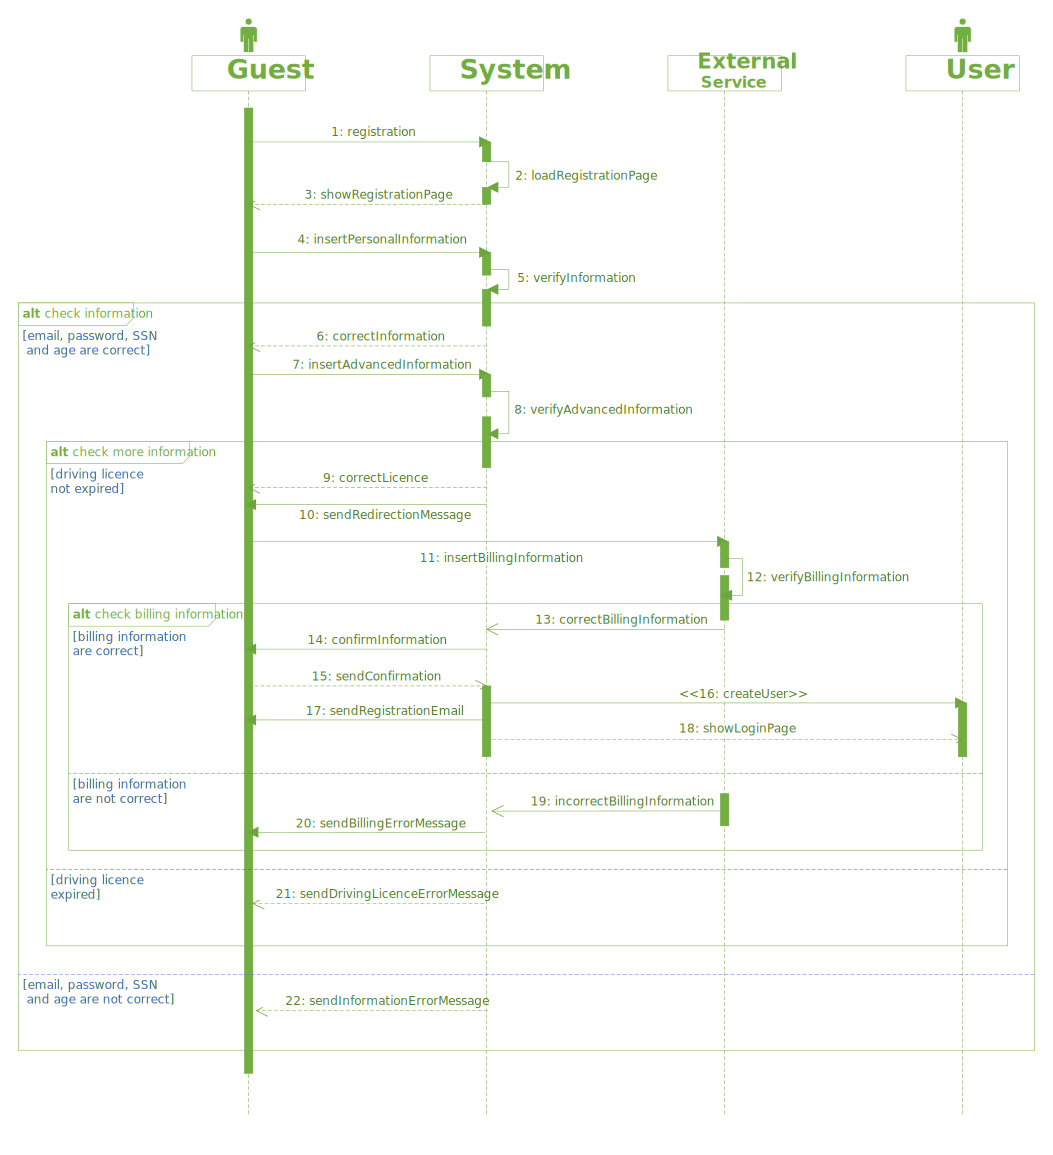
\includegraphics[width=1\textwidth,height=1\textheight,keepaspectratio]{res/img/seqdia_reg}
\par\end{centering}
\caption{Registration Sequence Diagram}
\end{figure}

\newpage{}

\begin{figure}[H]
\begin{centering}
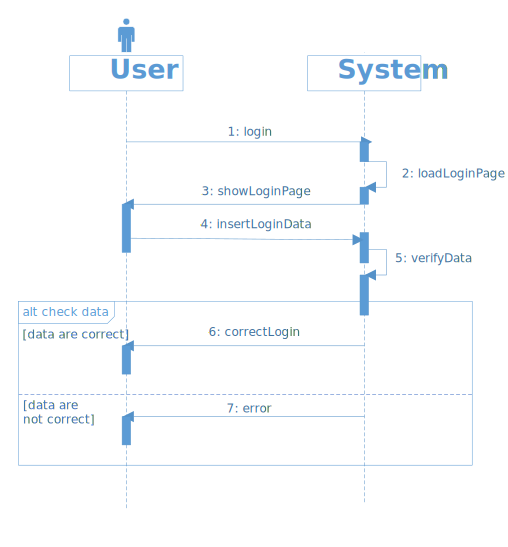
\includegraphics[width=0.7\textwidth,height=0.7\textheight,keepaspectratio]{res/img/seqdia_login}
\par\end{centering}
\caption{Login Sequence Diagram}
\end{figure}

\newpage{}

\begin{figure}[H]
\begin{centering}
\includegraphics[width=1\textwidth,height=0.9\textheight,keepaspectratio]{res/img/seqdia_checkavailability}
\par\end{centering}
\caption{Check Cars' Availability Sequence Diagram}
\end{figure}

\newpage{}

\begin{figure}[H]
\begin{centering}
\includegraphics[width=1\textwidth,height=0.7\textheight,keepaspectratio]{res/img/seqdia_editinfo}
\par\end{centering}
\caption{Modify Personal Information Sequence Diagram}
\end{figure}

\newpage{}

\begin{figure}[H]
\begin{centering}
\includegraphics[width=1\textwidth,height=1\textheight,keepaspectratio]{res/img/seqdia_editbilling}
\par\end{centering}
\caption{Modify Billing Information Sequence Diagram}
\end{figure}

\newpage{}

\begin{figure}[H]
\begin{centering}
\includegraphics[width=1\textwidth,height=1\textheight,keepaspectratio]{res/img/seqdia_reservation}
\par\end{centering}
\caption{ Car Reservation Sequence Diagram}
\end{figure}

\newpage{}

\begin{figure}[H]
\begin{centering}
\includegraphics[width=1\textwidth,height=1\textheight,keepaspectratio]{res/img/seqdia_opencar}
\par\end{centering}
\caption{Car Unlock Sequence Diagram}
\end{figure}

\newpage{}

\begin{figure}[H]
\begin{centering}
\includegraphics[width=1\textwidth,height=1\textheight]{res/img/seqdia_rent}
\par\end{centering}
\caption{Car Rental Sequence Diagram}
\end{figure}

\newpage{}

\begin{figure}[H]
\begin{centering}
\includegraphics[width=1\textwidth,height=1\textheight,keepaspectratio]{res/img/seqdia_contact}
\par\end{centering}
\caption{Contact Customer Service Sequence Diagram}
\end{figure}

\newpage{}

\subsection{Class Diagram}

Here it is shown a class diagram in order to give a static sight of
the main involved entities and of their relations. The diagram, whose
aim is just to better specificy requirements, is shown in this picture.

\quad{}

\begin{figure}[H]
\begin{centering}
\includegraphics[width=1\textwidth,height=1\textheight,keepaspectratio]{res/img/ClassD}
\par\end{centering}
\caption{Class Diagram}
\end{figure}

\newpage{}

\section{Alloy}

In this section we tried to verify the consistency of our class diagram.
To this goal, we realized a formal model of the system based both
on the class diagram and in the previously done assumptions and considerations
about constraints. We realized this model using Alloy syntax, thanks
to which we get on formally describing the domain of our application
and its properties. Then we verified the consistency of our model
using Alloy Analyzer. Here there is the code of the model of the system.

\quad{}

\lstdefinelanguage{alloy}
{keywords={%
      assert, pred, all, no, lone, one, some, check, run,
      but, let, implies, not, iff, in, and, or, set, sig, Int, int,
if, then, else, exactly, disj, fact, fun, module, abstract,
      extends, open, none, univ, iden, seq,
  },
  literate=%
    {:}{$\colon\ $}1
	%{|}{$\bullet$}1
    {==}{$=$}1
    {=}{$=\ $}1
    {!=}{$\neq\ $}1
    {&&}{$\land$}1
    {||}{$\lor\ $}1
    {<=}{$\le\ $}1
    {>=}{$\ge\ $}1
    %{all}{$\forall\ $}1
    {exists}{$\exists\ $}1
    {!in}{$\not\in\ $}1
    {\\in}{$\in$}1
    {=>}{$\implies\ $}2
    % the following isn't actually Alloy, but it gives the option to produce nicer latex
    {|=>}{$\Rightarrow$}2
    {<=set}{$\subseteq$}1
    {+set}{$\cup$}1
    {*set}{$\cap$}1
    {==>}{$\Longrightarrow$}3
    {<==>}{$\Longleftrightarrow$}4
    {...}{$\ldots$}1
    {\\hl}{$\hline$}1
    {\\alpha}{$\alpha$}1
    {\\beta}{$\beta$}1
    {\\gamma}{$\gamma$}1
    {\\delta}{$\delta$}1
    {\\epsilon}{$\epsilon$}1
    {\\zeta}{$\zeta$}1
    {\\eta}{$\eta$}1
    {\\theta}{$\theta$}1
    {\\iota}{$\iota$}1
    {\\kappa}{$\kappa$}1
    {\\lambda}{$\lambda$}1
    {\\mu}{$\mu$}1
    {\\nu}{$\nu$}1
    {\\xi}{$\xi$}1
    {\\pi}{$\pi$}1
    {\\rho}{$\rho$}1
    {\\sigma}{$\sigma$}1
    {\\tau}{$\tau$}1
    {\\upsilon}{$\upsilon$}1
    {\\phi}{$\phi$}1
    {\\chi}{$\chi$}1
    {\\psi}{$\psi$}1
    {\\omega}{$\omega$}1
    {\\Gamma}{$\Gamma$}1
    {\\Delta}{$\Delta$}1
    {\\Theta}{$\Theta$}1
    {\\Lambda}{$\Lambda$}1
    {\\Xi}{$\Xi$}1
    {\\Pi}{$\Pi$}1
    {\\Sigma}{$\Sigma$}1
    {\\Upsilon}{$\Upsilon$}1
    {\\Phi}{$\Phi$}1
    {\\Psi}{$\Psi$}1
    {\\Omega}{$\Omega$}1
    {\\EOF}{\;}1
    ,
  sensitive=true, % case sensitive
  morecomment=[l]//,%   
  morecomment=[l]{--},%
  morecomment=[s]{/*}{*/},%
  morestring=[b]",
  numbers=none,
  firstnumber=1,
  numberstyle=\tiny,
  stepnumber=2,
  basicstyle=\scriptsize\ttfamily\large,
  commentstyle=\bfseries\color{blue!20!black!50!green},
  keywordstyle=\bfseries\color{blue},
  numberstyle=\bfseries\color{red},
  ndkeywordstyle=\bfseries\color{red},
  tabsize=2,
  columns=fullflexible,
}
% inline
\def\A{%
    \lstinline[language=alloy,basicstyle=\ttfamily,columns=fixed]}

% paragraph
\lstnewenvironment{alloy}[1][]{%
  \lstset{language=alloy,
    floatplacement={tbp},captionpos=b,
    xleftmargin=8pt,xrightmargin=8pt,basicstyle=\ttfamily,#1}}{}

% paragraph from file
\newcommand{\alloyfile}[1]{
  \lstinputlisting[language=alloy,%
    frame=lines,xleftmargin=8pt,xrightmargin=8pt,basicstyle=\ttfamily,columns=fixed]{#1}

}
\lstinputlisting[language=alloy]{res/alloy/AlloyPowerEnjoy.als}  

\newpage{}

\subsection{Generated Worlds }

Here are presented three generated worlds, according to the model
specified in Alloy.

\includepdf[angle=90]{res/img/alloy_mondo_1}

\newpage{}

\includepdf[angle=90]{res/img/alloy_mondo_3}

\newpage{}

\includepdf[angle=90]{res/img/alloy_mondo_2}

\section{Appendix}

\subsection{Tools used}

We used the following tools to produce this document:
\begin{itemize}
\item \textbf{LaTex} as typesetting system to write this document
\item \textbf{LyX} as editor
\item \textbf{Visio Professional} to draw all the diagrams
\item \textbf{Alloy Analyzer 4.2} to write and verify alloy models
\end{itemize}

\subsection{Hours spent}

\begin{figure}[H]
\begin{centering}
\includegraphics[width=0.5\textwidth,height=0.5\textheight,keepaspectratio]{res/img/hours}
\par\end{centering}
\pagebreak{}
\end{figure}

\end{document}
